\section{Pattern matching equalities}
\label{spatmat}

For any node variables $a, b \in \Upsilon$ and $b, d$ terms, just by pattern matching, we have:  

\begin{figure}[h]
   \centerline{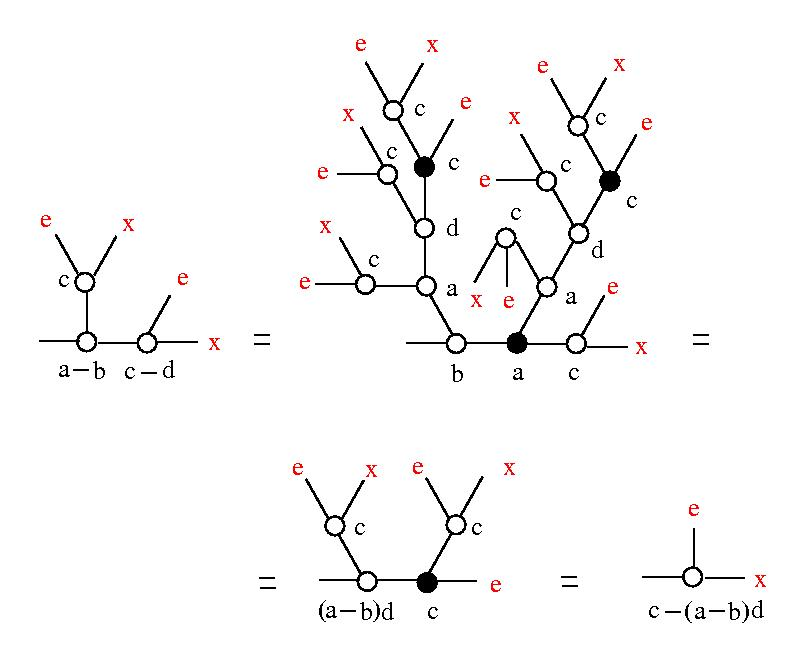
\includegraphics[width=100mm]{jpg/accept_4.jpg}}
\caption{ c-(a-b)d }
\label{fig1}
\end{figure}

Remark that the multiplication is obviously associative, i.e. $(ab)c = a(bc)$ for any terms $a, b, c$.



Let's see what this could mean. For expository purposes let's take $\Upsilon = (0,1)$ and the edge variables collection $X$ to be a real vector space. (As well we could take 
$$\displaystyle \Upsilon \, = \,  \left\{ a \in \mathbb{C}^{*} \mbox{ : } \mid a \mid < 1 \right\}$$ and $X$ a complex vector space. Later we shall see that these are only very particular examples of a general phenomenon.) Define further $\displaystyle a^{x}y = (1-a)x + ay$, or graphically: 
\vspace{.5cm} 
\centerline{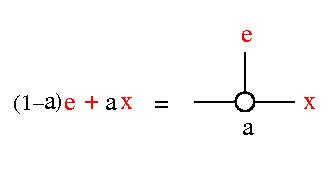
\includegraphics[width=50mm]{jpg/accept_0_1.jpg}} \vspace{.5cm}
and $\displaystyle \bar{a}=a^{-1}$. Then, for $a, b \in \Upsilon$ and $e, x \in X$ we have, by Definition \ref{ddifprod}
$$ (a-b)^{e} x \, = \,  b^{a^{e} x} \,  \bar{a}^{a^{e} x} e \, = \, (1-b) ((1-a) e + a x) + b ((1-a^{-1})((1-a)e + a x) + a^{-1}e) \, = \, $$ 
$$ = \, (1-b) ((1-a) e + a x) + b ((2-a)e + (a-1)x) \, = \, $$ $$ = \, ((1-b)(1-a) + b(2-a)) e + ((1-b)a + b(a-1))x \, = \, $$ 
$$ =\, (1-a+b)e + (a-b)x
$$ 
which motivates, in this very particular example, the reason behind the definition of the term $a-b$. A similar, but simpler computation for the product, is: 
$$(ab)^{e} x \, = \, a^{e} \, b^{e} x \, = \, (1-a) e + a((1-b)e + bx) \, = \, (1-ab)e + ab x$$
We can check that $$\displaystyle 0^{e} x \, = \, (1-0) e + 0 x = e$$  $$\displaystyle 1^{e} x \, = \, \bar{1}^{e} x \,  = \, (1-1)e + 1 x \, = \, x$$

The equality from the Figure (\ref{fig1}) where we used pattern matching is then (for $a, b, c, d \in \Upsilon$): 
$$ (a-b)^{c^{e} x} \, (c-d)^{e} x \, = \, (c-(a-b)d)^{e} x $$
which is indeed true, because
$$(a-b)^{c^{e} x} \, (c-d)^{e} x \, = \, (1-a+b) ((1-c) e + c x) + (a-b) ((1-c+d) e + (c-d)x) = \, $$ 
$$ = \, ((1-a+b)(1-c) + (a-b)(1-c+d)) e + ((1-a+b)c + (a-b)(c-d)) x \, = \,$$
$$ = \,  (1-c-a+ac+b-bc+a-b-ac+bc+ad-bd) e + (c-ac+bc+ac-bc-ad+bd)x \, = $$ 
$$ = \, (1-c+ad-bd) e + (c-ad+bd)x$$
and 
$\displaystyle (c-(a-b)d)^{e} x \, = \, = (c-ad+bd)^{e} x \, = \, (1-c+ad-bd) e + (c-ad+bd)x$. 

\vspace{.5cm}

\paragraph{Discussion.} We can prove (in Figure \ref{a-0-fig}) by pattern matching that, in general, for any $a \in \Upsilon$ 
\begin{figure}[h] \centerline{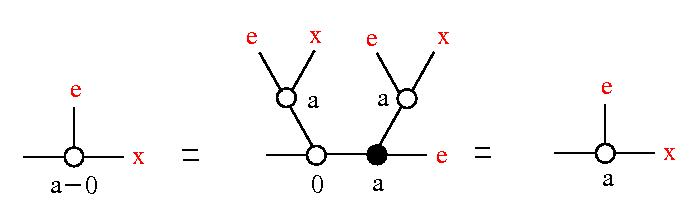
\includegraphics[width=110mm]{jpg/a-0.jpg}}  \caption{ $a-0 = a$ by pattern matching} \label{a-0-fig} \end{figure}
\begin{equation}
(a-0)^{e} x \,  = \, a^{e} x
\label{a-0}
\end{equation}
But we can't prove (in Figure \ref{a0-fig}) that  for any $a \in \Upsilon$ 
\begin{equation}
(a 0)^{e} x \,  = \, 0^{e} x \, = \, e
\label{a0}
\end{equation}
\begin{figure}[h] \centerline{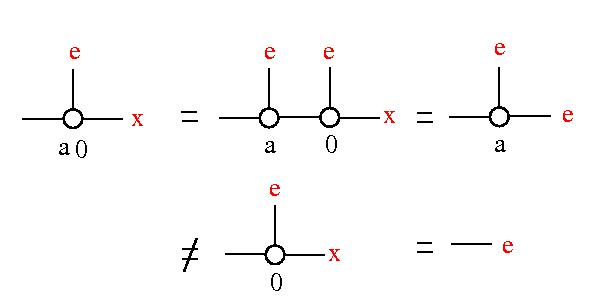
\includegraphics[width=100mm]{jpg/a0.jpg}}
\caption{ $a 0 \not = 0$ by pattern matching }
\label{a0-fig}
\end{figure}




In general, we can't prove by pattern matching only equalities like (\ref{a-a}) or (\ref{a-(a-b)}). 
\begin{equation}
(a-a)^{e} x \,  = \, 0^{e} x \, = \, e
\label{a-a}
\end{equation}

\begin{equation}
(a-(a-b))^{e} x \, =\, b^{e} x
\label{a-(a-b)}
\end{equation}
for any node variable $a \in \Upsilon$ and any binary term $b$.  

Indeed, Figure \ref{a-a-fig} shows this for (\ref{a-a}).  More interestingly, if we try to prove (\ref{a-(a-b)}) by pattern matching, like in Figure \ref{a-(a-b)-fig}, then at some point we are stuck without something like (\ref{a-a}) to use. 

\begin{figure}[h]\centerline{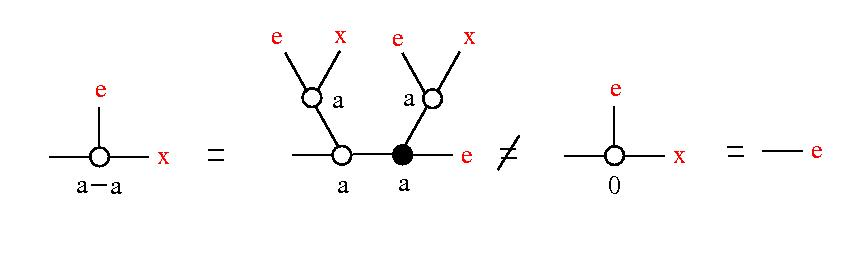
\includegraphics[width=120mm]{jpg/a-a.jpg}}  \caption{ $a-a \not = 0$ by pattern matching } \label{a-a-fig}  
\end{figure}

\begin{figure}[h]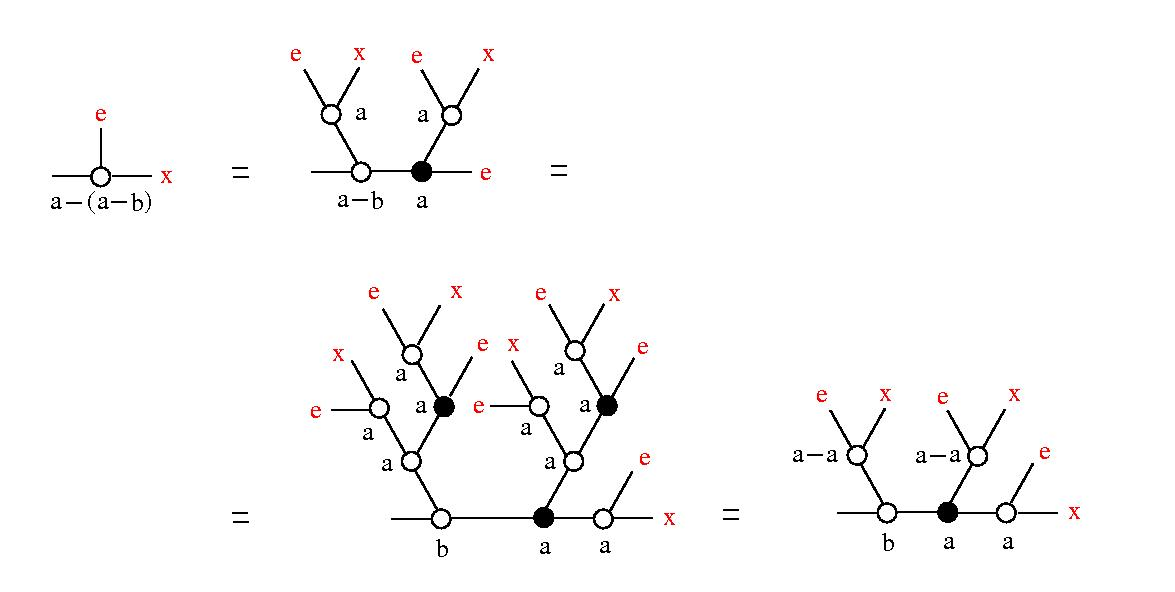
\includegraphics[width=120mm]{jpg/a-a-b.jpg}  \caption{ $a-(a-b) \not = b$ by pattern matching } \label{a-(a-b)-fig} \end{figure}




Another problem concerns the commutativity of multiplication. There is no reason for it in general. Remark for example that in Figure (\ref{fig1}) we wrote $(a-b)d$, where $a$ is a node variable and $b, d$ are terms. It is not true that $(a-b)d = d(a-b)$. The Figure \ref{a-bd-fig} shows that. 
\begin{figure}[h]\centerline{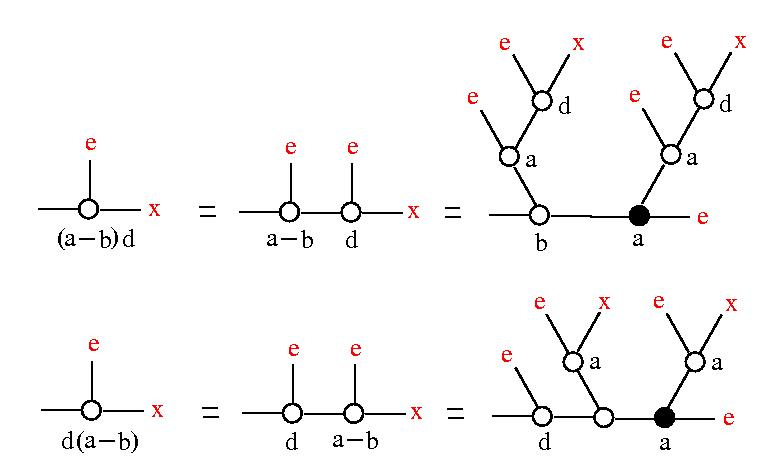
\includegraphics[width=100mm]{jpg/a-bd.jpg}}
\caption{ $(a-b)d \not = d(a-b)$ by pattern matching} \label{a-bd-fig} 
\end{figure}


Even for $a, b \in \Upsilon$ node variables, it is not true that 
\begin{equation}
(a b)^{e} x \, = (b a)^{e} x
\label{abba}
\end{equation}
\begin{equation}
(a \bar{b})^{e} x \, = (\bar{b}a)^{e} x
\label{abbara}
\end{equation}
\begin{equation}
(\bar{a} \bar{b})^{e} x \, = (\bar{b} \bar{a})^{e} x
\label{barabbara}
\end{equation}

With the choices made in the particular example, all  these equalities are trivially true and some of them are also equalities which we'd wish to have in general. But we don't have them by pattern matching only.

